\documentclass{sigchi}

% Use this command to override the default ACM copyright statement (e.g. for preprints). 
% Consult the conference website for the camera-ready copyright statement.


%% EXAMPLE BEGIN -- HOW TO OVERRIDE THE DEFAULT COPYRIGHT STRIP -- (July 22, 2013 - Paul Baumann)
% \toappear{Permission to make digital or hard copies of all or part of this work for personal or classroom use is 	granted without fee provided that copies are not made or distributed for profit or commercial advantage and that copies bear this notice and the full citation on the first page. Copyrights for components of this work owned by others than ACM must be honored. Abstracting with credit is permitted. To copy otherwise, or republish, to post on servers or to redistribute to lists, requires prior specific permission and/or a fee. Request permissions from permissions@acm.org. \\
% {\emph{CHI'14}}, April 26--May 1, 2014, Toronto, Canada. \\
% Copyright \copyright~2014 ACM ISBN/14/04...\$15.00. \\
% DOI string from ACM form confirmation}
%% EXAMPLE END -- HOW TO OVERRIDE THE DEFAULT COPYRIGHT STRIP -- (July 22, 2013 - Paul Baumann)


% Arabic page numbers for submission. 
% Remove this line to eliminate page numbers for the camera ready copy
\pagenumbering{arabic}


% Load basic packages
\usepackage{balance}  % to better equalize the last page
\usepackage{graphics} % for EPS, load graphicx instead
\usepackage{times}    % comment if you want LaTeX's default font
\usepackage{url}      % llt: nicely formatted URLs
\usepackage{wrapfig}



% llt: Define a global style for URLs, rather that the default one
\makeatletter
\def\url@leostyle{%
  \@ifundefined{selectfont}{\def\UrlFont{\sf}}{\def\UrlFont{\small\bf\ttfamily}}}
\makeatother
\urlstyle{leo}


% To make various LaTeX processors do the right thing with page size.
\def\pprw{8.5in}
\def\pprh{11in}
\special{papersize=\pprw,\pprh}
\setlength{\paperwidth}{\pprw}
\setlength{\paperheight}{\pprh}
\setlength{\pdfpagewidth}{\pprw}
\setlength{\pdfpageheight}{\pprh}

% Make sure hyperref comes last of your loaded packages, 
% to give it a fighting chance of not being over-written, 
% since its job is to redefine many LaTeX commands.
\usepackage[pdftex]{hyperref}
\hypersetup{
pdftitle={GlassmanUISTPosterAbstract},
pdfauthor={LaTeX},
pdfkeywords={UIST, Posters},
bookmarksnumbered,
pdfstartview={FitH},
colorlinks,
citecolor=black,
filecolor=black,
linkcolor=black,
urlcolor=black,
breaklinks=true,
}

% create a shortcut to typeset table headings
\newcommand\tabhead[1]{\small\textbf{#1}}


% End of preamble. Here it comes the document.
\begin{document}

\title{OverCode: Visualizing Variation in Student Solutions to Programming Problems at Scale}

\numberofauthors{5}
\author{
  \alignauthor Elena Leah Glassman\\
    \affaddr{MIT CSAIL}\\
    \email{elg@mit.edu}
  \alignauthor Jeremy Scott\\
    \affaddr{MIT CSAIL}\\
    \email{jks@mit.edu}
  \alignauthor Rishabh Singh\\
    \affaddr{MIT CSAIL}\\
    \email{rishabh@csail.mit.edu}
      \alignauthor Philip Guo\\
      \affaddr{MIT CSAIL,}\\
      \affaddr{University of Rochester}\\
      \email{pg@cs.rochester.edu}
            \alignauthor Robert C. Miller\\
      \affaddr{MIT CSAIL}\\
      \email{rcm@mit.edu}
}


\maketitle

\begin{abstract}
In MOOCs, a single programming exercise may produce thousands of solutions from learners. Understanding solution variation is important for providing appropriate feedback to students at scale.  The wide variation among these solutions can be a source of pedagogically valuable examples, and can be used to refine the autograder for the exercise by exposing corner cases. 
We present OverCode, a system for visualizing and exploring thousands of programming solutions. OverCode uses both static and dynamic analysis to cluster similar solutions, and lets instructors further filter and cluster solutions based on different criteria.
We evaluated OverCode against a non-clustering baseline in a within-subjects study with 24 teaching assistants, and found that the OverCode interface allows teachers to more quickly develop a high-level view of students' understanding and misconceptions, and to provide feedback that is relevant to more students.
\end{abstract}

\category{H.5.m.}{Information Interfaces and Presentation (e.g. HCI)}{Miscellaneous}

\section{Introduction}

Intelligent tutoring systems (ITSes), Massive Open Online Courses (MOOCs), and websites like Khan Academy and Codecademy are now used to teach programming courses at a massive scale. In these courses, a single programming exercise may produce thousands of solutions from learners, which presents both an opportunity and a challenge. For teachers, the wide variation among these solutions can be a source of pedagogically valuable examples~\cite{marton13}, and understanding this variation is important for providing appropriate, tailored feedback to students~\cite{basupowergrading,MOOCshop}. The variation can also be useful for refining evaluation rubrics, since it can expose corner cases in automatic grading tests.

Sifting through thousands of solutions to understand their variation and find pedagogically valuable examples is a daunting task, even if the programming exercises are simple and the solutions are only tens of lines of code long. Without tool support, a teacher may not read more than 50-100 of them before growing frustrated with the tedium of the task. Given this small sample size, teachers cannot be expected to develop a thorough understanding of the variety of strategies used to solve the problem, or produce instructive feedback that is relevant to a large proportion of learners, or find unexpected interesting solutions.

An information visualization approach would enable teachers to explore the variation in solutions at scale. Existing techniques~\cite{gradingsigcse14,MOOCshop,codewebs} use a combination of clustering to group solutions that are semantically similar, and graph visualization to show the variation between these clusters. These clustering algorithms perform pairwise comparisons that are quadratic in both the number of solutions and in the size of each solution, which scales poorly to thousands of solutions. Graph visualization also struggles with how to label the graph node for a cluster, because it has been formed by a complex combination of code features. Without meaningful labels for clusters in the graph, the rich information of the learners' solutions is lost and the teacher's ability to understand variation is weakened.

\begin{figure}
\centering
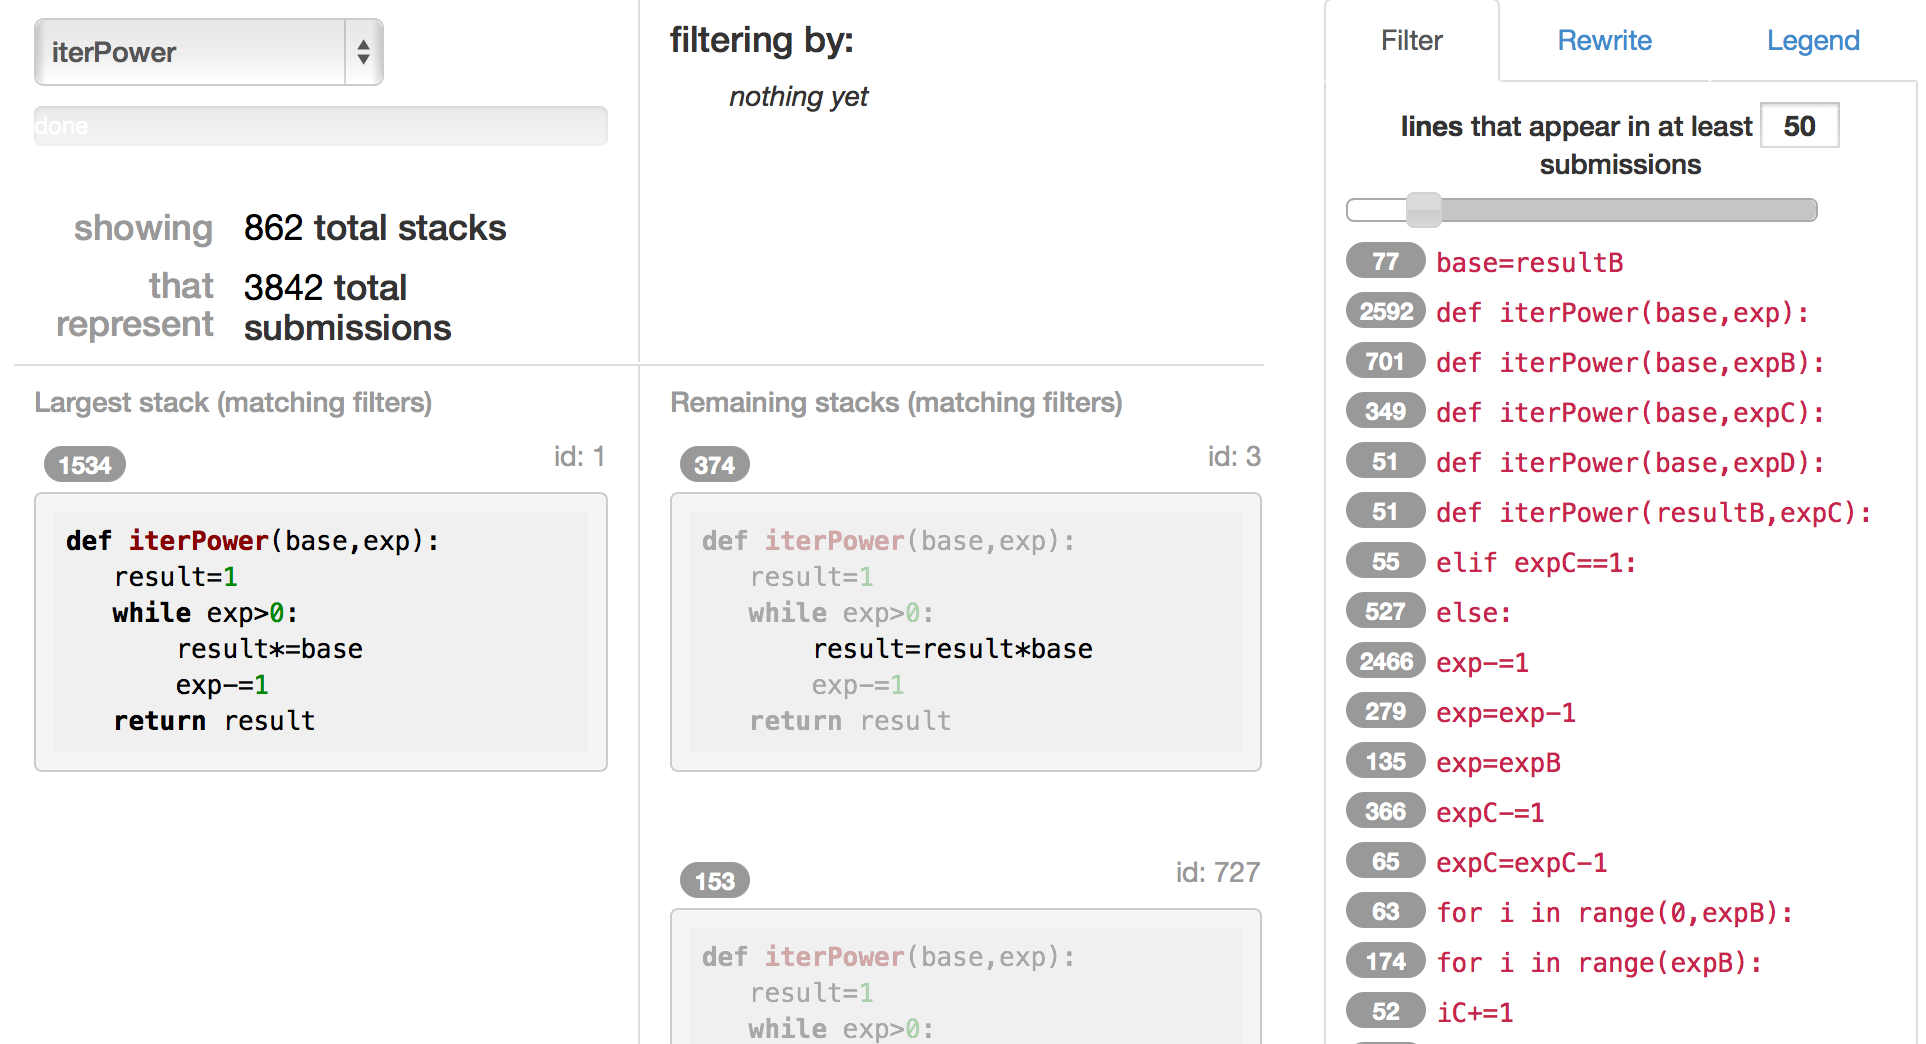
\includegraphics[width=0.5\textwidth]{frontPageInterfacePreview.png}
\caption{OverCode user interface.}
\label{fig:figure1}
\end{figure}
% We created a code clustering technique that scales linearly with the number of solutions.
%An important design principle of OverCode is that the clusters of student solutions are represented as readable, executable code that describes every solution in that cluster. , for each cluster,

In this poster we present OverCode, a system for visualizing and exploring the variation in thousands of programming solutions.  OverCode is designed to visualize correct solutions, in the sense that they pass the automatic grading tests typically used in a programming class at scale.  OverCode uses a novel clustering technique that creates clusters of identical cleaned code, is time linear in both the number of solutions and the size of each solution. The cleaned code is readable, executable, and describes every solution in that cluster.  The cleaned code is shown in a visualization that puts code front-and-center (Figure~\ref{fig:figure1}). In OverCode, the teacher reads through code solutions that each represent an entire cluster of solutions that look and act the same. The differences between clusters are highlighted to help instructors discover and understand the variations among submitted solutions. Clusters can be filtered by the lines of code within them.  Clusters can also be merged together with {\em rewrite rules} that collapse variations that the teacher decides are unimportant. 

A cluster in OverCode is a set of solutions that perform the same computations, but may use different variable names or statement order.  OverCode uses a lightweight dynamic analysis to generate clusters, which scales linearly with the number of solutions. It clusters solutions whose variables take the same sequence of values when executed on test inputs and whose set of constituent lines of code are syntactically the same. An important component of this analysis is to rename variables that behave the same across different solutions. The renaming of variables serves three main purposes. First, it lets teachers create a mental mapping between variable names and their behavior which is consistent across the entire set of solutions. This may reduce the cognitive load for a teacher to understand different solutions. Second, it helps clustering by reducing variation between similar solutions. Finally, it also helps make the remaining differences between different solutions more salient. 

In two user studies with a total of 24 participants, we compared the OverCode interface with a baseline interface that showed original unclustered solutions. When using OverCode, participants felt that they were able to develop a better high-level view of the students' understandings and misconceptions. While participants didn't necessarily read more lines of code in the OverCode interface than in the baseline, the code they did read came from clusters containing a greater percentage of all the submitted solutions. Participants also drafted mock class forum posts about common good and bad solutions that were relevant to more solutions (and the students who wrote them) when using OverCode as compared to the baseline. 

The main contributions of this work are:
\begin{itemize}
\item a novel visualization that shows similarity and variation among thousands of solutions, with cleaned code shown for each variant. 
\item an algorithm that uses the behavior of variables to help cluster solutions and generate the cleaned code for each cluster of solutions.
\item two user studies that show this visualization is useful for giving instructors a bird's-eye view of thousands of students' solutions.
\end{itemize}

\section{Summary}
We have designed the OverCode system for visualizing thousands of Python programming solutions to help instructors explore the variations among them. Unlike previous approaches, OverCode uses a lightweight static and dynamic analysis to generate stacks of similar solutions and uses variable renaming to present cleaned solutions for each stack in an interactive user interface. It allows instructors to filter stacks by line occurrence and to further merge different stacks by composing rewrite rules. Based on two user studies with 24 current and potential teaching assistants, we found OverCode allowed instructors to more quickly develop a high-level view of students' understanding and misconceptions, and provide feedback that is relevant to more students. We believe an information visualization approach is necessary for instructors to explore the variations among solutions at the scale of MOOCs, and OverCode is an important step towards that goal. 	

\section{Acknowledgments}

This material is based, in part, upon work supported by the National Science Foundation Graduate Research Fellowship (grant 1122374), the Microsoft Research Fellowship, the Bose Foundation Fellowship, and by Quanta Computer as part of the Qmulus Project. Any opinions, findings, conclusions, or recommendations in this paper are the authors', and do not necessarily reflect the views of the sponsors.


% Balancing columns in a ref list is a bit of a pain because you
% either use a hack like flushend or balance, or manually insert
% a column break.  http://www.tex.ac.uk/cgi-bin/texfaq2html?label=balance
% multicols doesn't work because we're already in two-column mode,
% and flushend isn't awesome, so I choose balance.  See this
% for more info: http://cs.brown.edu/system/software/latex/doc/balance.pdf
%
% Note that in a perfect world balance wants to be in the first
% column of the last page.
%
% If balance doesn't work for you, you can remove that and
% hard-code a column break into the bbl file right before you
% submit:
%
% http://stackoverflow.com/questions/2149854/how-to-manually-equalize-columns-
% in-an-ieee-paper-if-using-bibtex
%
% Or, just remove \balance and give up on balancing the last page.
%
\balance


\bibliographystyle{acm-sigchi}
\bibliography{icerbib}
\end{document}



